\chapter{Whose Eyes? Observers in Motion}
\label{ch:xobs}

A black-hole image depends on who takes it. Two observers passing the same
point at different velocities see the same light arrive from different
directions (aberration), at different frequencies (Doppler shift) and with
different brightness (beaming). Their clocks also run at different rates
relative to a distant observer's. The thesis' camera was always a static
observer far away, for whom none of this matters. This chapter gives the
camera a 4-velocity.

\section{Observers and their frames}

A camera is an observer with 4-velocity $u = e_0$ and an orthonormal spatial
triad $e_i$. A pixel looking along the unit direction $n$ receives the photon
with $k \propto e_0 - n^i e_i$, which the tracer follows backward
(thesis Appendix on image handedness). The reference observer at each point
is the zero-angular-momentum observer (ZAMO) of \citet{BardeenPressTeukolsky1972},
\begin{equation}
e_{\hat t} = \frac{1}{\alpha}\left(\partial_t + \omega\,\partial_\phi\right),
\qquad
\alpha = \sqrt{-g_{tt} + g_{t\phi}^2/g_{\phi\phi}}, \quad
\omega = -\frac{g_{t\phi}}{g_{\phi\phi}},
\end{equation}
with the spatial legs along the BL coordinate directions, normalised. An
observer moving with velocity $\vec v$ relative to the ZAMO has the
Lorentz-boosted tetrad
\begin{equation}
e_0' = \gamma\,(e_{\hat t} + v^j e_{\hat j}), \qquad
e_i' = e_{\hat i} + \frac{\gamma - 1}{v^2}\,v_i\,(v^j e_{\hat j}) + \gamma\,v_i\,e_{\hat t},
\label{eq:boost}
\end{equation}
orthonormal by construction. Aberration, Doppler shift and beaming of
everything the camera sees then follow from tracing the received photons.
Nothing is added by hand. The clock rate against far-away time is
$d\tau/dt = 1/e_0'^{\,t}$.

The simulator offers five observers (\texttt{sgr\_physics/observers.hpp},
shared by the renderer and the validation tools):
\begin{description}
\item[ZAMO:] $\vec v = 0$, the frame-dragged observer.
\item[Orbiting:] circulating at the prograde Keplerian rate
$\Omega = 1/(r^{3/2} + a)$, so $v_{\hat\phi} = (\Omega - \omega)\sqrt{g_{\phi\phi}}/\alpha$.
This is a geodesic only on the equator.
\item[Free fall:] falling from rest at infinity with $E = 1$, $L_z = Q = 0$
--- the ``rain'' frame of \citet{HamiltonLisle2008} --- with
$v_{\hat r} = -\sqrt{2Mr(r^2+a^2)/A}$. For this observer $\gamma = 1/\alpha$
exactly and there is no polar motion.
\item[Hovering:] at rest relative to the distant stars ($u \propto
\partial_t$), so $v_{\hat\phi} = -\omega\sqrt{g_{\phi\phi}}/\alpha$. This
observer needs a rocket, and becomes impossible ($v \to c$) at the
ergosphere $r_E(\theta) = M + \sqrt{M^2 - a^2\cos^2\theta}$.
\item[Riding an S-star:] the star's coordinate velocity from its full-GR
orbit, the same orbit model the thesis fits to the data (S2 passes
pericentre at about 2.5 per cent of light speed, \citealp{Gravity2018}).
\end{description}

The test suite (\texttt{test\_observers.cpp}) checks these closed forms:
\begin{itemize}
\item every tetrad is orthonormal to $10^{-12}$;
\item the orbiting observer's $u^t$, $E$ and $L$ are those of the BPT72
circular orbit;
\item the free-fall observer has $u_t = -1$ and $u_\phi = 0$ at every
$(r, \theta)$;
\item the hovering observer's $u^t$ is $1/\sqrt{-g_{tt}}$;
\item hovering is valid at $1.001\,r_E$ and invalid at $0.999\,r_E$.
\end{itemize}

\section{Clocks and speeds}

Table~\ref{tab:xobs} lists each observer's speed relative to the local ZAMO
and its clock rate at three radii on the equator. The Schwarzschild entries
reproduce textbook values: at the ISCO ($r = 6M$) the circular orbit moves at
$\XIscoSpeedSchw\,c$ and its clock runs at $d\tau/dt = \XIscoClockSchw =
1/\sqrt2$, and the free-falling clock runs at $\alpha^2 = 1 - 2M/r$. For
\sgra's spin the hovering observer at $6M$ must already move at
$\XHoverSpeedSix\,c$ against the frame dragging just to stay still. The
free-falling observer reaches $\XInfallSpeedHorizon\,c$ relative to the ZAMO
at $1.001\,r_+$ ($r_+ = \XRplus\,M$).

\begin{table}
\centering
\caption{Speed $v$ relative to the local ZAMO [$c$] and clock rate
$d\tau/dt$ (observer proper time per unit far-away time) of the four
standard observers on the equator (\texttt{observer\_tool}).}
\label{tab:xobs}
\small
% AUTO-GENERATED by scripts/make_numbers_ext.py — do not edit by hand.
\begin{tabular}{rr cc cc cc cc}
\toprule
& & \multicolumn{2}{c}{ZAMO} & \multicolumn{2}{c}{orbiting} & \multicolumn{2}{c}{free fall} & \multicolumn{2}{c}{hovering} \\
$\astar$ & $r/M$ & $v$ & $d\tau/dt$ & $v$ & $d\tau/dt$ & $v$ & $d\tau/dt$ & $v$ & $d\tau/dt$ \\
\midrule
0 & 60 & 0.000 & 0.9832 & 0.131 & 0.9747 & 0.183 & 0.9667 & 0.000 & 0.9832 \\
0 & 15 & 0.000 & 0.9309 & 0.277 & 0.8944 & 0.365 & 0.8667 & 0.000 & 0.9309 \\
0 & 6 & 0.000 & 0.8165 & 0.500 & 0.7071 & 0.577 & 0.6667 & 0.000 & 0.8165 \\
0.94 & 60 & 0.000 & 0.9832 & 0.131 & 0.9748 & 0.183 & 0.9667 & 0.001 & 0.9832 \\
0.94 & 15 & 0.000 & 0.9310 & 0.265 & 0.8978 & 0.365 & 0.8667 & 0.009 & 0.9309 \\
0.94 & 6 & 0.000 & 0.8181 & 0.414 & 0.7448 & 0.575 & 0.6693 & 0.063 & 0.8165 \\
\bottomrule
\end{tabular}

\end{table}

\section{What they see}
\label{sec:xaberration}

Figure~\ref{fig:xobsrenders} shows the same place --- the camera position
of the close-orbit scene (Table~\ref{tab:xpresets}) --- through three
observers' eyes. The free-falling
observer sees the shadow and disk shrink toward the direction of motion and
brighten and blue-shift: light from ahead is aberrated forward. The orbiting
observer sees the whole scene displaced toward its direction of motion,
brighter ahead and dimmer behind.

\begin{figure}
\centering
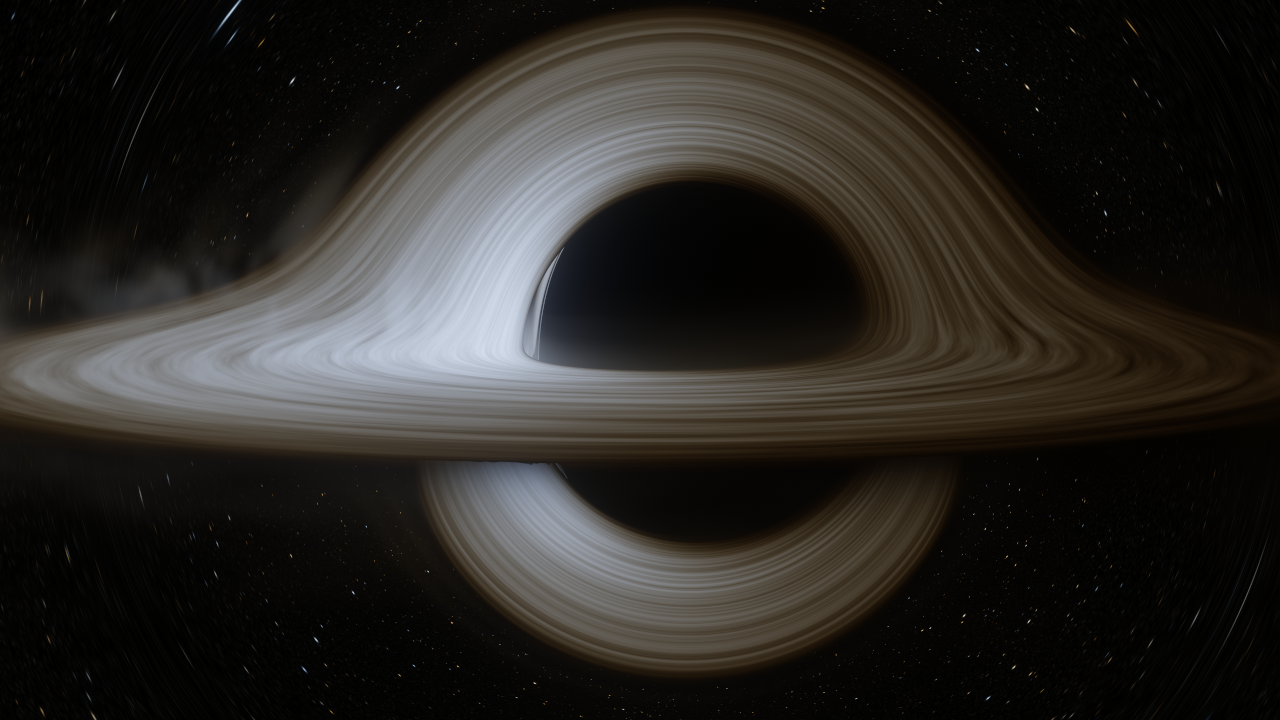
\includegraphics[width=0.32\textwidth]{figures/x_obs_zamo.png}\hfill
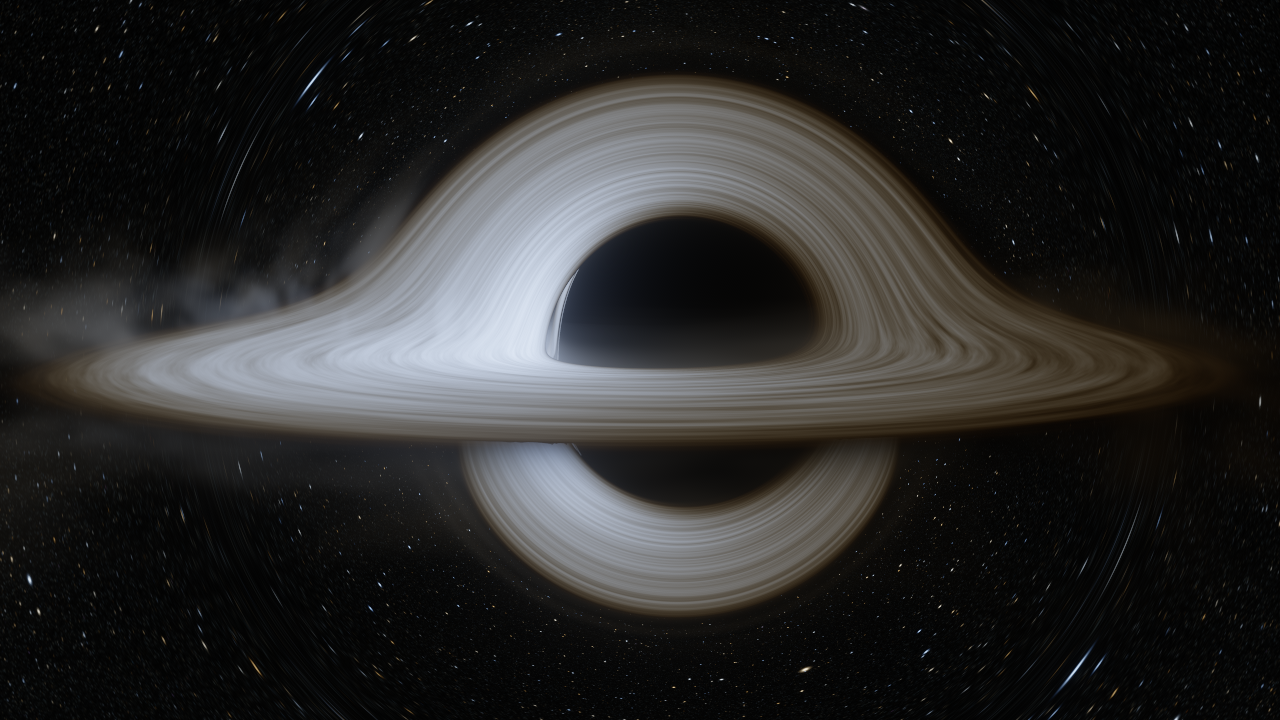
\includegraphics[width=0.32\textwidth]{figures/x_obs_infall.png}\hfill
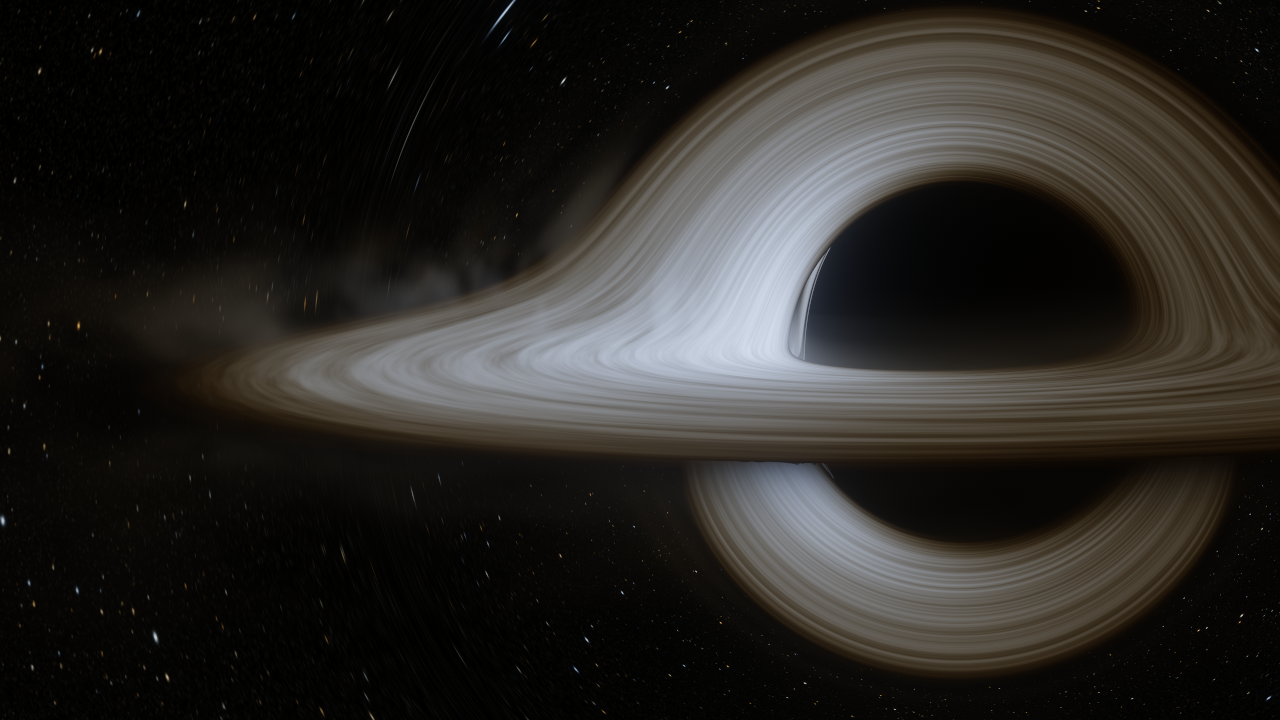
\includegraphics[width=0.32\textwidth]{figures/x_obs_orbit.png}
\caption{One place, three observers: the close-orbit scene seen by a ZAMO
(left), by an observer falling from rest at infinity (centre) and by one
orbiting at the Keplerian rate (right). Only the camera's tetrad differs.}
\label{fig:xobsrenders}
\end{figure}

The shadow makes these effects quantitative because its edge has a closed
form in the Schwarzschild case. A static observer at radius $r$ sees a
circular shadow of angular radius $\sin\psi = 3\sqrt3\,M\sqrt{1 - 2M/r}/r$
\citep{Synge1966}, which is $\XSyngeDeg\degr$ at $r = 10\,M$. A moving observer
sees every direction aberrated, $\cos\chi' = (\cos\chi + v)/(1 + v\cos\chi)$
for the angle $\chi$ to its velocity. Bisecting the shadow edges on the fp64
Kerr--Schild tracer with each observer's tetrad (\texttt{observer\_tool})
reproduces this prediction to $\XAberrationCheck$ in the tangent of the edge
angle:
\begin{itemize}
\item the free-falling observer ($v = \XInfallSpeedTen$) sees a shadow of
radius $\XInfallEdgeDeg\degr$;
\item the orbiting observer ($v = \XOrbitSpeedTen$) sees its edges at
$\XOrbitEdgeLeftDeg\degr$ on the trailing side and $\XOrbitEdgeRightDeg\degr$
on the leading side.
\end{itemize}
At $\astar = 0.94$ the ZAMO's shadow is already lopsided, with edges at
$\XKerrZamoLeftDeg\degr$ (prograde) and $\XKerrZamoRightDeg\degr$. The
orbiting observer's aberration carries the whole shadow past the centre of
view, to between $\XKerrOrbitLeftDeg\degr$ and $\XKerrOrbitRightDeg\degr$ on
the leading side (Fig.~\ref{fig:xedges}).

\begin{figure}
\centering
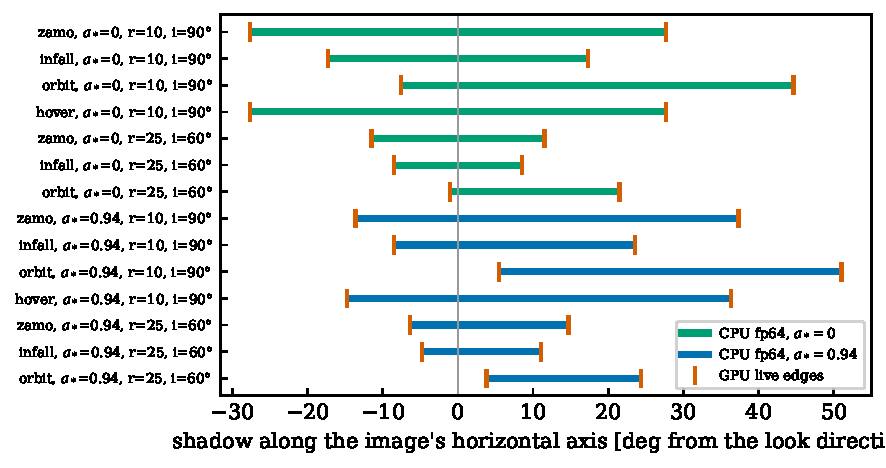
\includegraphics[width=0.85\textwidth]{figures/fig_x_observer_edges.pdf}
\caption{The shadow along the image's horizontal axis for each observer and
camera position (bars: fp64 Kerr--Schild bisection; ticks: the live GPU
renderer). At $\astar = 0$ the bars equal Synge's shadow aberrated by the
observer's velocity.}
\label{fig:xedges}
\end{figure}

\section{The sky they see}

The background shifts too. For a backward ray normalised so the camera
measures unit frequency, the conserved $p_t$ gives the ratio of received to
emitted frequency for light from infinity, $g_{\rm sky} = 1/p_t$. Deep in the
potential the sky is blueshifted by $1/\alpha$ for a ZAMO, more ahead of a
falling observer and less behind it. The renderer applies this shift to the
Milky Way map using the 6500\,K blackbody approximation of
\S\ref{sec:sky}. The effect is weak for these exterior observers, but it
dominates the view near the horizon (Chapter~\ref{ch:xinfall}).

\section{Frame dragging made visible}

Inside the ergosphere nothing can remain at rest relative to the stars, and
light is dragged too. Every captured ray crosses the ergosurface, so tinting
those rays would only colour the shadow. The overlay instead marks the light
that went \emph{inside} $r_E$ and still escaped. That set is not symmetric. At
$\astar = 0.94$ the prograde equatorial photon orbit, at $\XRphPro\,M$, lies
inside the ergosphere ($\XRergoEq\,M$ on the equator), while the retrograde
one, at $\XRphRetro\,M$, lies outside it. Only light passing on the prograde side can visit
the ergoregion and return, and it does so in a thin crescent hugging that
side of the shadow (Fig.~\ref{fig:xergo}). The crescent is a direct picture
of frame dragging.

\begin{figure}
\centering
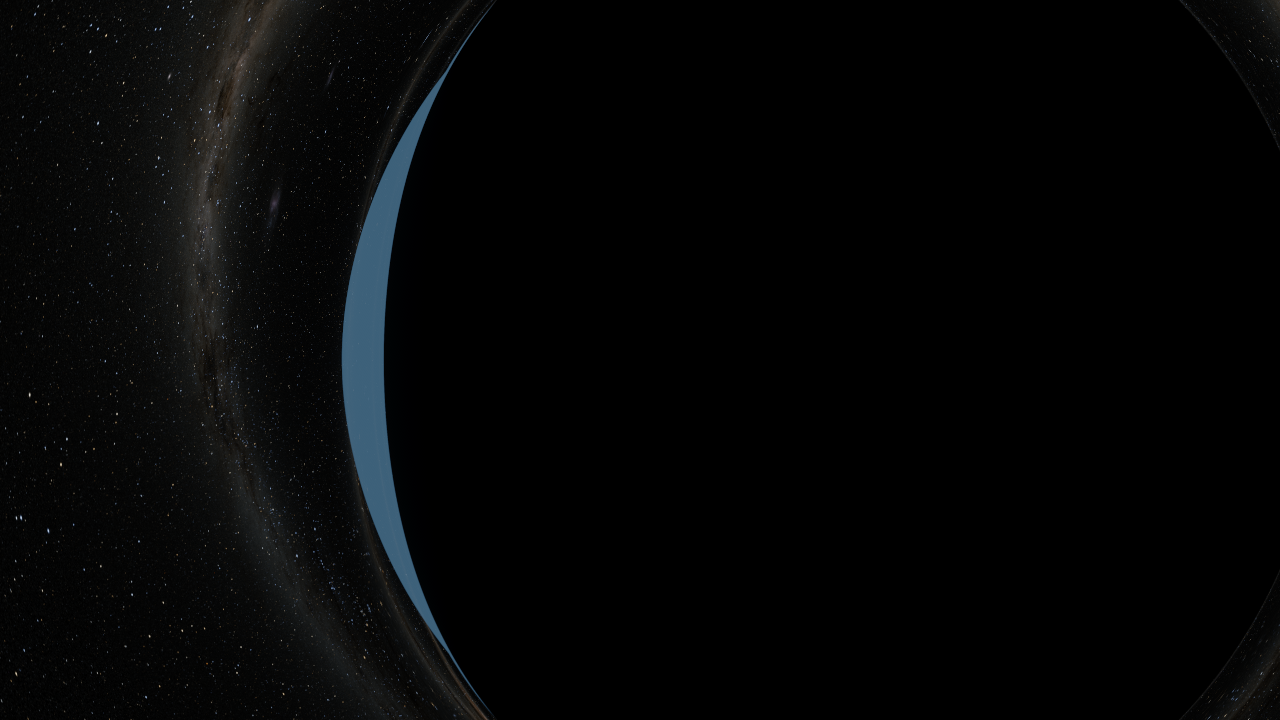
\includegraphics[width=0.7\textwidth]{figures/x_ergo_crescent.png}
\caption{Light that passed through the ergoregion and escaped (blue overlay)
around \sgra{} seen nearly edge-on ($i = 88\degr$, $r = 30\,M$, no disk;
lensed Milky Way behind). Captured light is not marked. The crescent appears
only on the prograde side, where photon orbits dip inside the ergosphere.}
\label{fig:xergo}
\end{figure}

\section{Validating the live observers}
\label{sec:xobsgpu}

The live renderer receives the boosted tetrad~\eqref{eq:boost}, computed in
double precision by the same library function the CPU tools use and
expressed in Kerr--Schild components. \texttt{compare\_observers.py} renders a
one-pixel-high strip through the image centre against a uniform sky, with no
disk, so captured rays are exact zeros. It then compares the GPU shadow edges
with the fp64 edges for $\XObsGpuCases$ observer and spin configurations. The
largest difference is $\XObsGpuMaxPx$ pixel (one pixel is $\XObsGpuPixel$ in
the tangent of the angle).

That agreement came only after the comparison found a defect. The live
kernel gave each ray at most $\XLegacyBudgetSteps$ steps and counted a ray
that exhausted them as captured. Near the high-spin prograde photon orbit
($r = \XRphPro\,M$ at $\astar = 0.94$) the orbit is only weakly unstable. A ray one
pixel from the shadow edge winds several times at about a thousand steps per
orbit, ran out of budget, and was wrongly darkened. Edge-on, this widened the
prograde side of the shadow by $\XLegacyBudgetPx$ pixels at the comparison's
resolution. The budget is now $\XBudgetSteps$ steps. Only rays at the photon ring use the
extra steps, and the old budget can be re-run on demand to reproduce the
record.
